%%******************************************************************************
%%
%% body01.tex
%%
%%******************************************************************************
%%
%% Title......: DORIS - Offshore Facilities Monitoring Robots
%%
%% Author.....: COPPE/LEAD-UFRJ Team - G2 (Embedded Electronics)
%%
%% Started....:      Fri Feb 01 2013
%% Last Modified...: Fri Jun 10 2013
%%
%% Emails.....: liu@coep.ufrj.br
%%              jacoud@poli.ufrj.br
%%              marco.fsantosx@gmail.com
%%              renan028@gmail.com
%%
%% Address....: Universidade Federal do Rio de Janeiro
%%              Caixa Postal 68.504, CEP: 21.945-970
%%              Rio de Janeiro, RJ - Brasil.
%%
%%******************************************************************************


%%******************************************************************************
%% CHAPTER - Preliminary Schemes and Definitions
%%******************************************************************************


\chapter{Supervisory Electronic Circuits}
In this chapter, it will be presented the schemes, drawings and explanations that illustrate DORIS preliminary electronics architecture and its subdivisions.


%%******************************************************************************
%% SECTION - Section
%%******************************************************************************


\section{Protection and Monitoring Circuits}
According to G3, the power supply of the entire robot will be generated by six battery packs. The batteries were specified so that they can supply the motors' power, thus providing a current peak of 18 amperes each. These batteries will also be used to supply the rest of the electronics architecture (devices, computers, microcontrollers, etc.), which demands less power than the motor system. Due to eventual short circuits, equipment fault and battery failures, excess currents can arise, which can cause damage to the equipment and generate excessive heat. In order to provide over-current protection, two solutions were investigated: a) utilization of electric fuses; b) active current limiting using transistors.\\
\\
Fuses are low resistance resistors that act as a sacrificial component, intentionally engineered to blow under over-current. The essential component of a fuse is a metal wire that melts as soon as an excessive current flows along it. Thus, the loop becomes opened; hence, devices in the circuit are protected. When the fuse blows, the protected equipment won't be energized until the fuse is replaced by another with same specification. In DORIS, protection circuits consist of individual electric fuse for each equipment, owing to different voltage/current specifications. A market survey of fuse models can be found in section XXXXX.\\
\\
Active current limiting circuit has fast response if compared to fuses and is not sacrificial (no need of electronic replacements in case of over-current). An example of a circuit schematic in figure~\ref{FIG:SUPCIRPROT} can be used to protect the output power transistor Q1 (called "output transistor"). The resistor R1 is the "load current sensing component", 0.5 ohm in the example. Q2 is the "protection transistor" which turns on as soon as the voltage across R1 becomes about 0.65 V. When Q2 turns on, it removes base current from Q1 thereby reducing the collector current of Q1. Neglecting the base currents of Q1 and Q2, the collector current of Q1 is also the load current. Thus, R1 fixes the maximum current to a value given by 0.65/R1 = 1.3 A, for any given output voltage and load resistance. The problem of this scheme is the power dissipation in transistor with current limiting, which could increase to about 60 W, hence requiring heat-sinks, which is very difficult to implement in DORIS structure.
\begin{figure}
  \centering
  % Requires \usepackage{graphicx}
  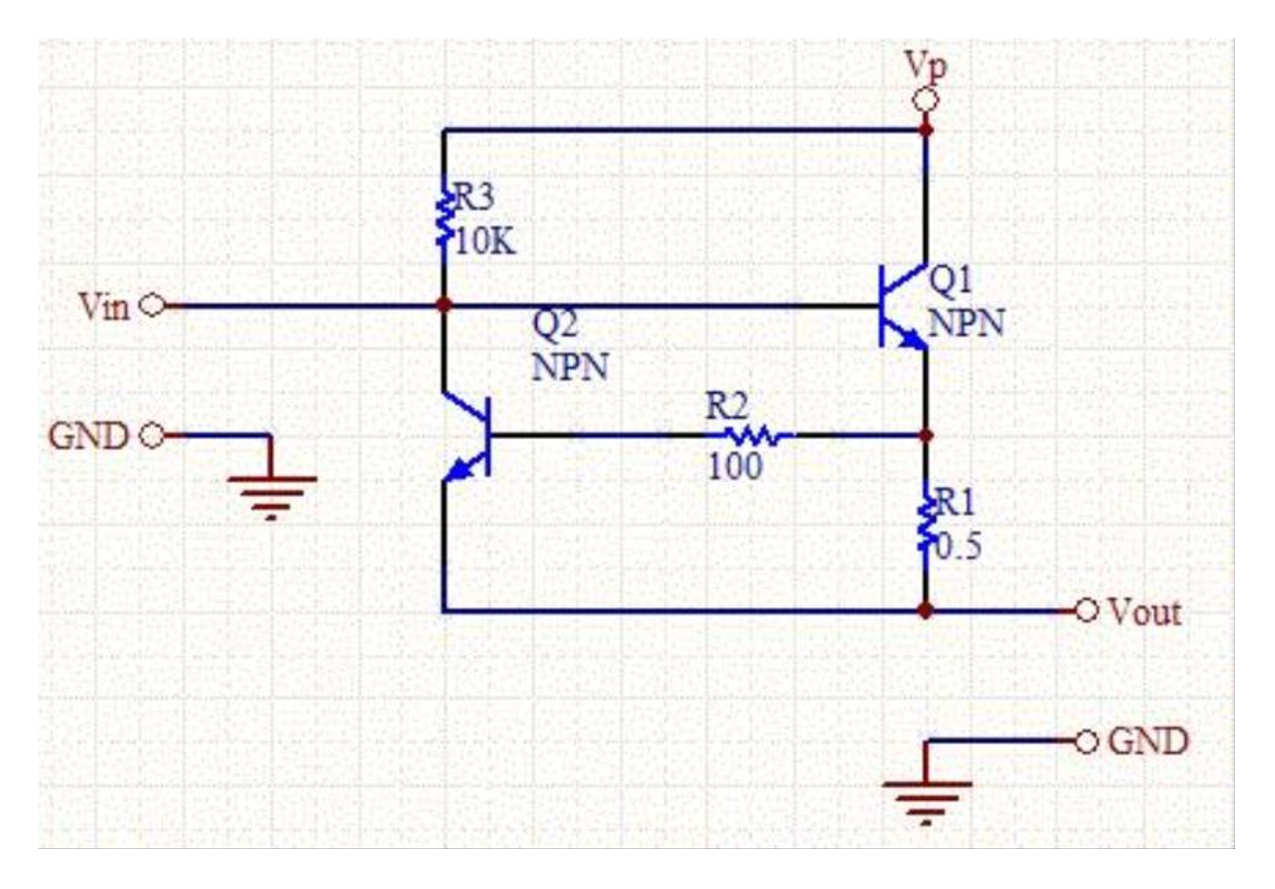
\includegraphics[width=1\columnwidth]{figs/tables/SupCirProt.pdf}\\
  \caption[Protection transistors]{Protection transistors.}
  \label{FIG:SUPCIRPROT}
\end{figure}
Besides current protection, equipment need be powered by a regular source, with the correct voltage specified by equipment. A DC/DC converter is a mechanism that is connected to a power source having its own internal impedance. This device converts an input voltage into an output voltage, making it possible to create the different levels needed in project. In each wagon of DORIS, three DC/DC converters will be installed: 24V to 5V, 12V and 24V. In addition, these devices also perform signal treatment before feeding the supply to the equipment. Motor drivers already have DC signal treatment; therefore they will be directly powered by the batteries.
Microcontrollers (one per module) will receive the voltages signals supplied to equipment and signals from wagon's temperature and humidity sensors. This information can be accessed via Ethernet by operator or embedded PC. This system is named "Monitoring Circuits", and it briefly consists of the microcontroller voltages and sensors signals analysis.\\
\\
In addition, the microcontrollers control the state of a set of relays, whose function is turn on/off the devices in case of emergency (device protection) or economic power consumption. The system with relays and fuses is named "Protection circuits". In figure~\ref{SUPCIRPROT2}, there is a block diagram of conceptual design of the protection and monitoring circuits. In figure XXXXX there is a scheme of the circuit and components.
\begin{figure}
  \centering
  % Requires \usepackage{graphicx}
  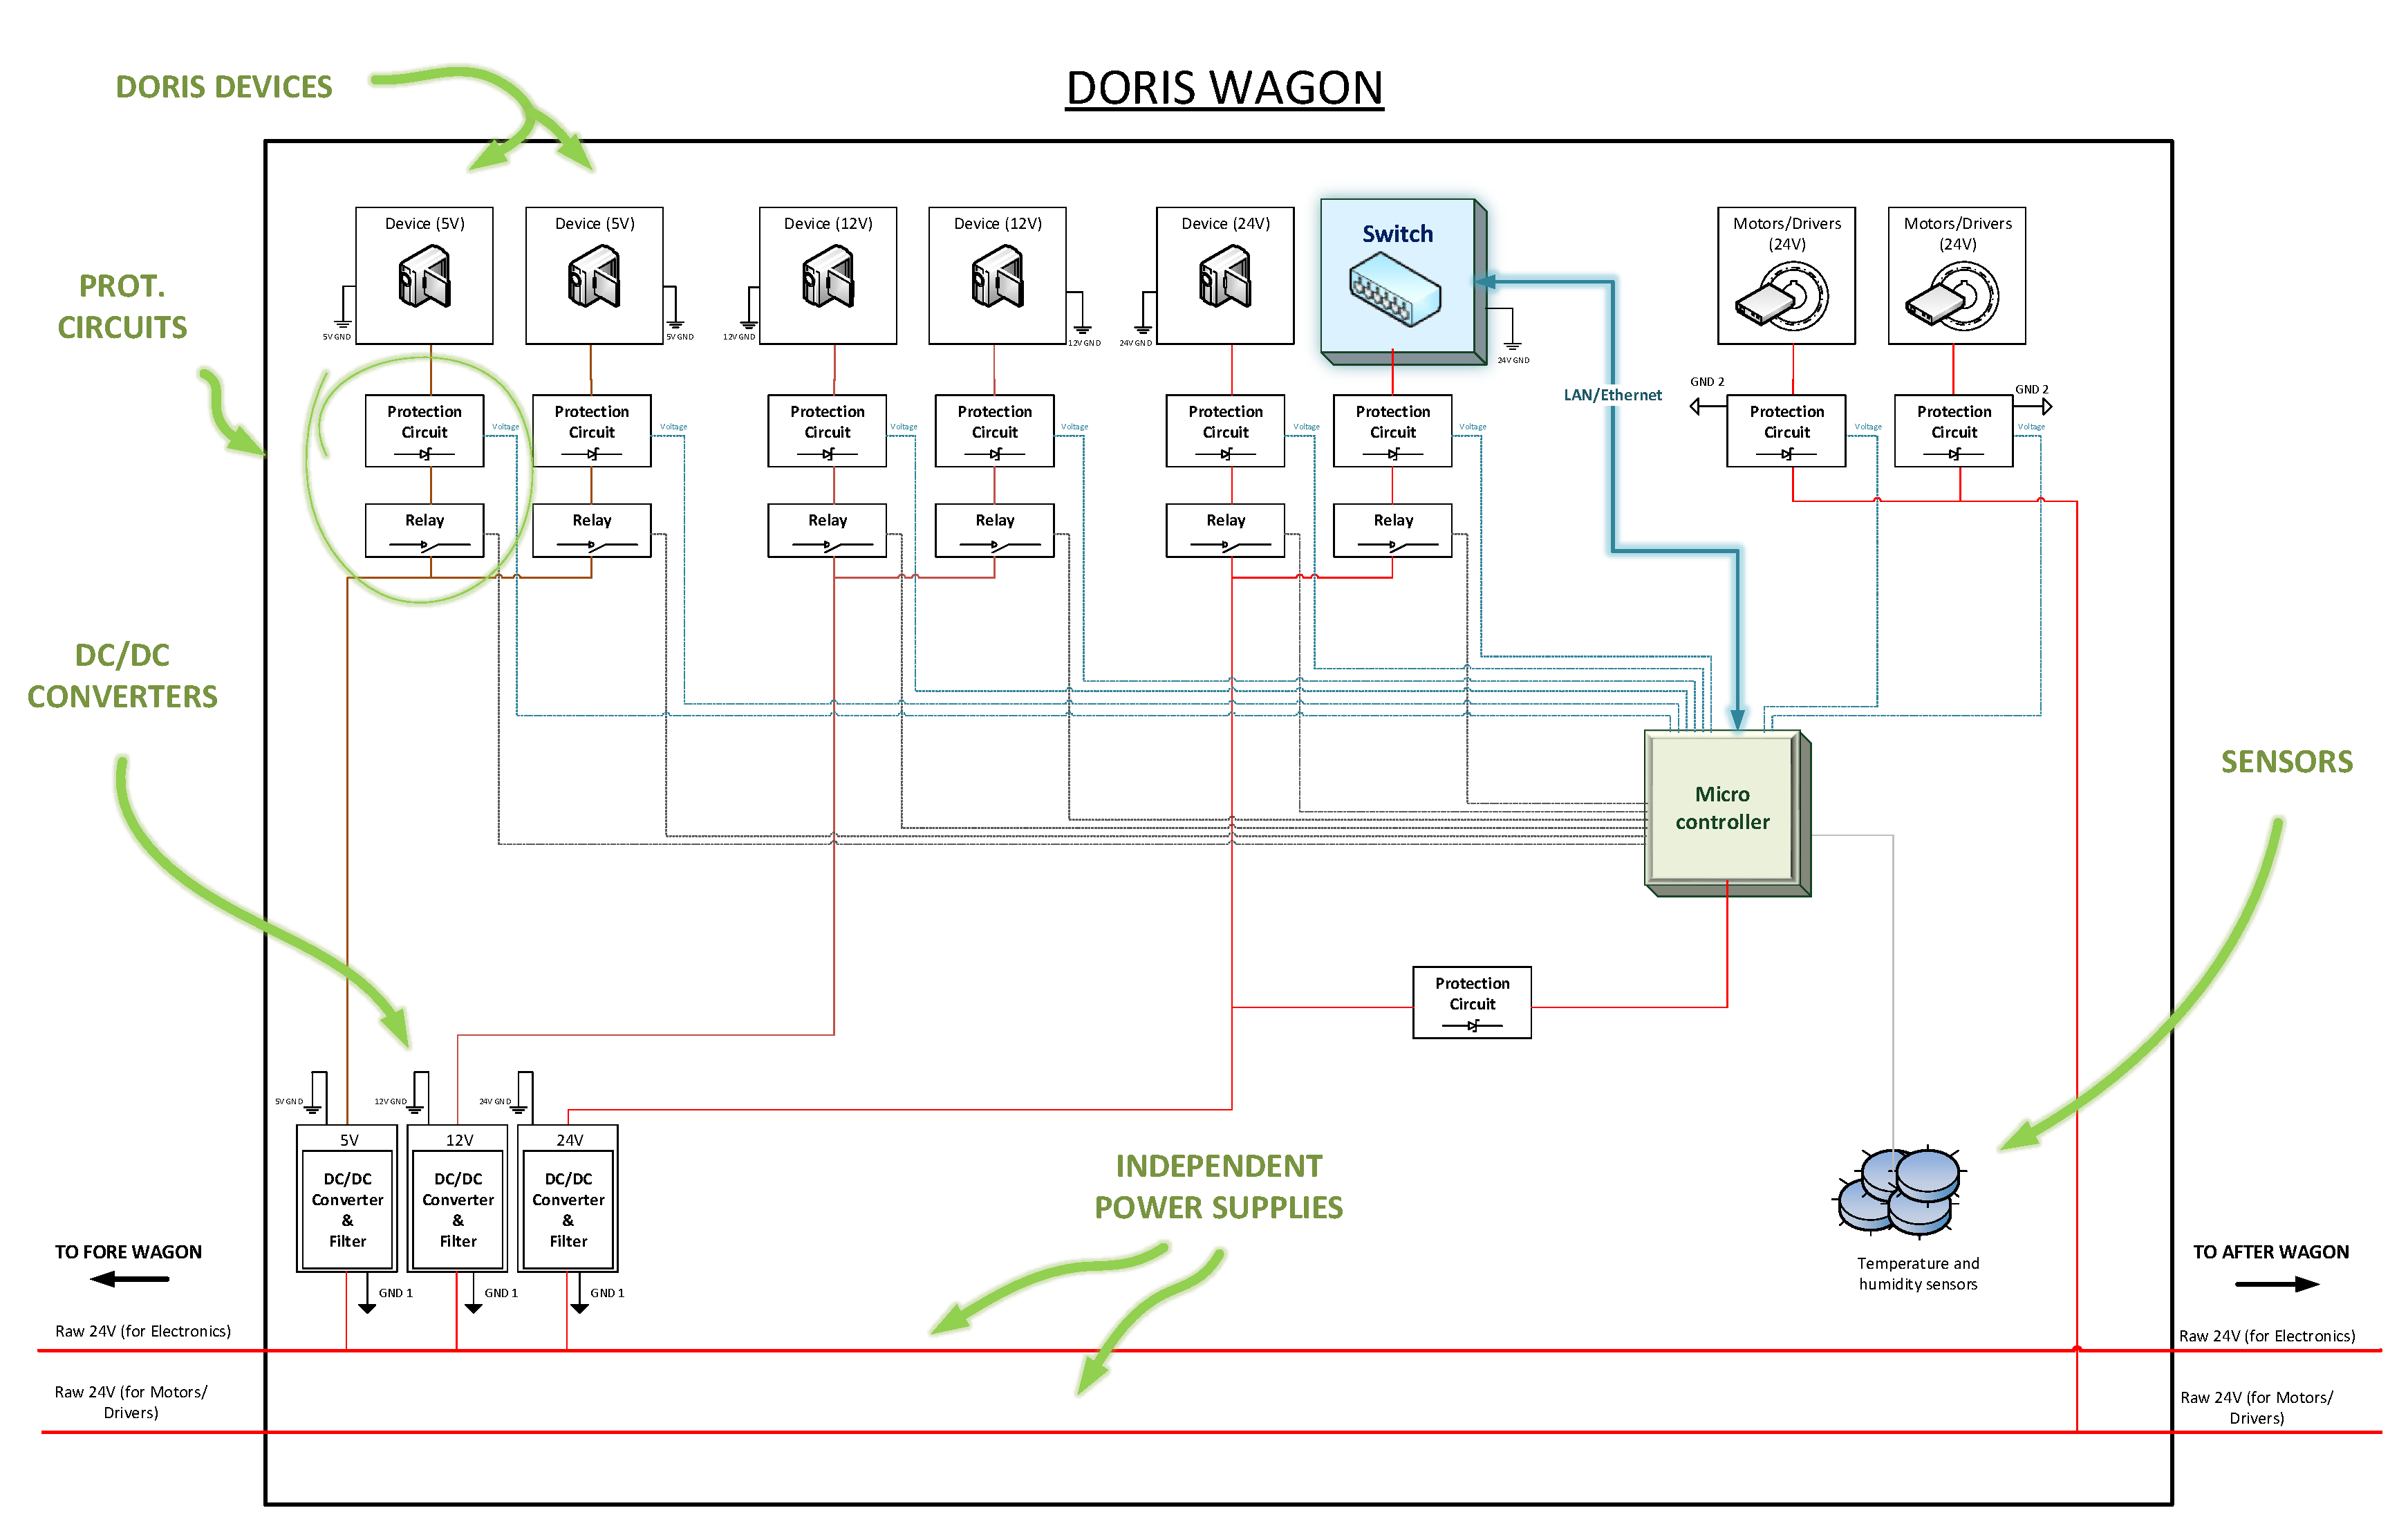
\includegraphics[width=1\columnwidth]{figs/tables/WagonPowerSupply.pdf}\\
  \caption[Block diagram of conceptual design of the protection and monitoring circuits]{Block diagram of conceptual design of the protection and monitoring circuits.}
  \label{FIG:SUPCIRPROT2}
\end{figure}
%----------------------------------------------------------------------------
\section{Robot Startup/Shutdown And Power Supply Management}
Hazardous and explosive environments demand heavy protection of robot modules and devices.  Also, some functionalities of the robot need to be available as much as possible, such as robot complete startup/shutdown and power supply management. As well as the other modules, in the power supply, a microcontroller will be accountable for electronics supervision: monitoring, protection, and in this case, battery management, selecting the best battery arrangement for DORIS power buses to better power performance.\\
\\
In emergency situations, such as rail damage, explosion or fire in robot route, or robot damage, DORIS should leave its position or stops its trajectory, which could reach the critical area. Thereby, the robot startup/shutdown function should always be available. The Wi-Fi solution may be unavailable due to range or infrastructure, thus other solutions have been investigated: physical button and an alternative wireless technology (radio).
The conceptual design of the physical button can be seen in figure~\ref{FIG:SUPCIRPS2}. If the physical button is pressed, the relay will close and the microcontroller accountable for power supply management will be un-powered. The entire robot will shut down and will not be possible to restart or communicate to it remotely. The operator will need to manually press the button again to access the robot remotely.
\begin{figure}
  \centering
  % Requires \usepackage{graphicx}
  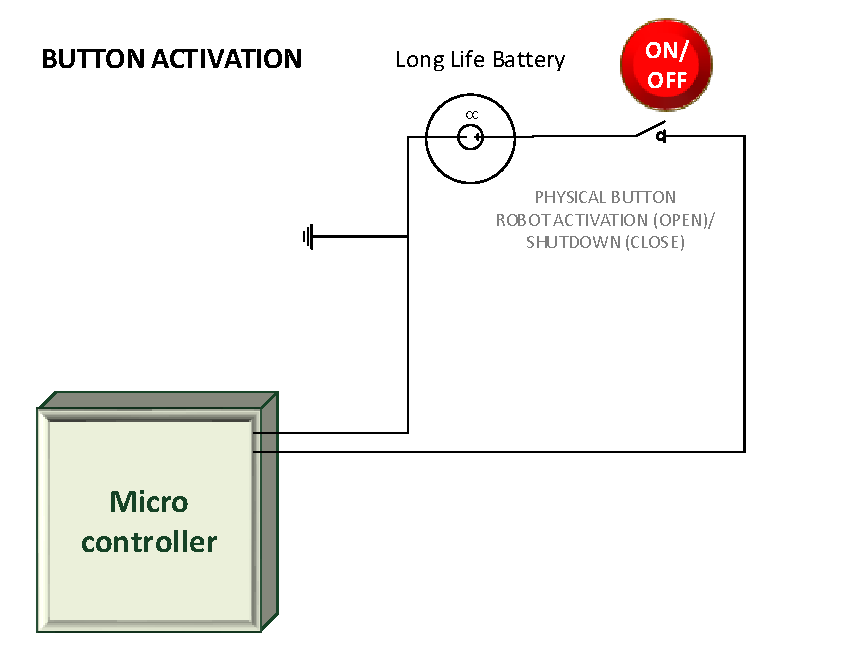
\includegraphics[width=1\columnwidth]{figs/tables/geralblockPS2.pdf}\\
  \caption[Conceptual design of the physical button]{Conceptual design of the physical button.}
  \label{FIG:SUPCIRPS2}
\end{figure}
Another solution for startup/shutdown function and remote operation is the utilization of an alternative wireless communication. The radio system is composed by a transmitter (base) and a receiver (robot), figure XXXXX. The first's electronic components are high power antenna, battery, buttons and relays. The second's electronic components are low power antenna, long cycle life battery, microcontroller and relays. In case of operator command, the receiver's microcontroller will deactivate the entire robot, using the logic gates of the power management system.\\
\\
The power management system's components, in power supply module, are: microcontrollers responsible for battery monitoring and managing, mechanical relays for battery switching and basic electronics (resistors, transistors, logic gates). The figure~\ref{FIG:SUPCIRPS1} shows its conceptual design. The power managing microcontroller receives batteries signals status via SMBUS, process and broadcast this information to the PCs via Ethernet ($I^2{C}$ adapter), and it actuates on the mechanical relays for battery switching. The mechanical relays, two for each battery, connect the batteries to the power buses of DORIS. The robot has six batteries in total and, in order to protect electronic devices of interferences (see power supply report), it has two independent power buses: the first for electronic devices, which consumes two batteries, and the second for drivers and motors, which requires three batteries (two backup batteries). The microcontroller chooses, via the mechanical relays, the batteries arrangement, i.e., the batteries connections with the power buses.
\begin{figure}
  \centering
  % Requires \usepackage{graphicx}
  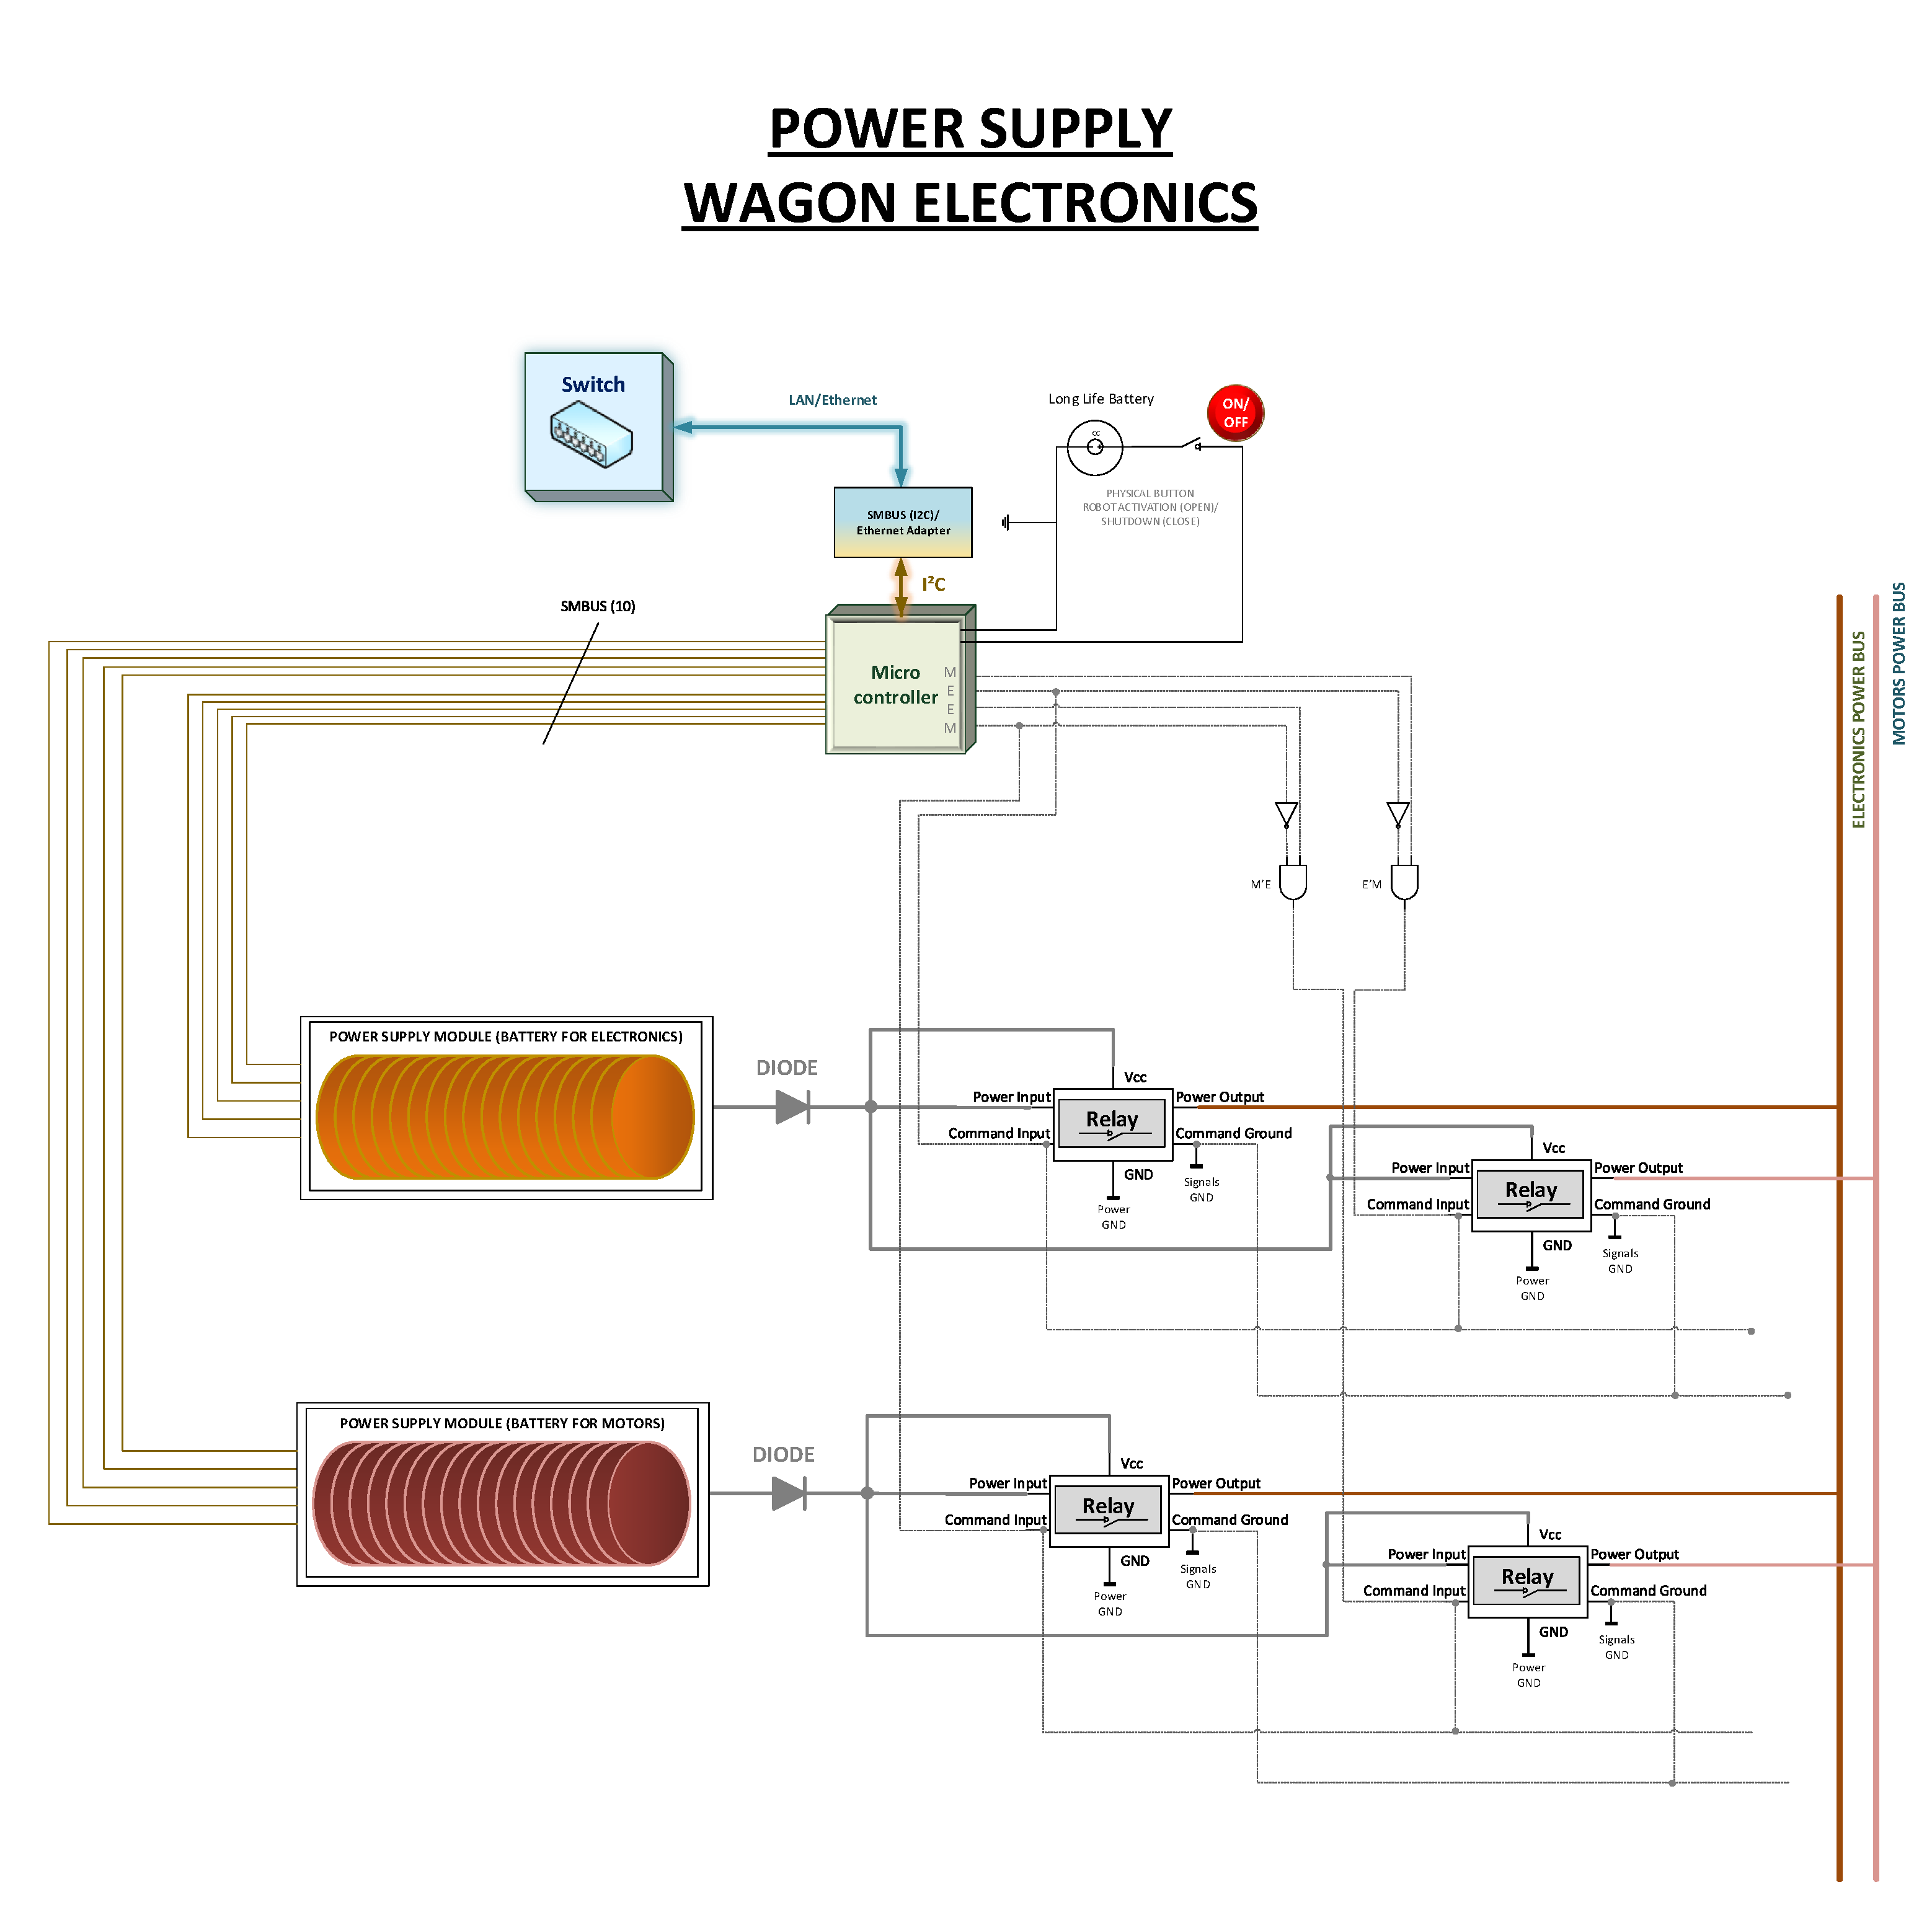
\includegraphics[width=1\columnwidth]{figs/tables/geralblockPS1.pdf}\\
  \caption[Conceptual design of power management system]{Conceptual design of power management system.}
  \label{FIG:SUPCIRPS1}
\end{figure}
The programming logic of the power managing microcontroller is not accessible by the operator for DORIS safety, but batteries status, such as temperature and level, will be available. The microcontroller must be capable of interpret this information to battery reconfiguration in case of emergencies or for power performance improvement. Also, logic gates protect batteries to be connected in both power buses, in case of microcontroller failure.\\
\\
In order to guarantee the power supply management, the microcontroller need to be powered all the time, requiring an independent long cycle life battery. To reduce the long cycle life battery power consumption, the mechanical relays will be activated pulling current of the DORIS batteries through transistor (see figure~\ref{FIG:SUPCIRPS3}.
\begin{figure}
  \centering
  % Requires \usepackage{graphicx}
  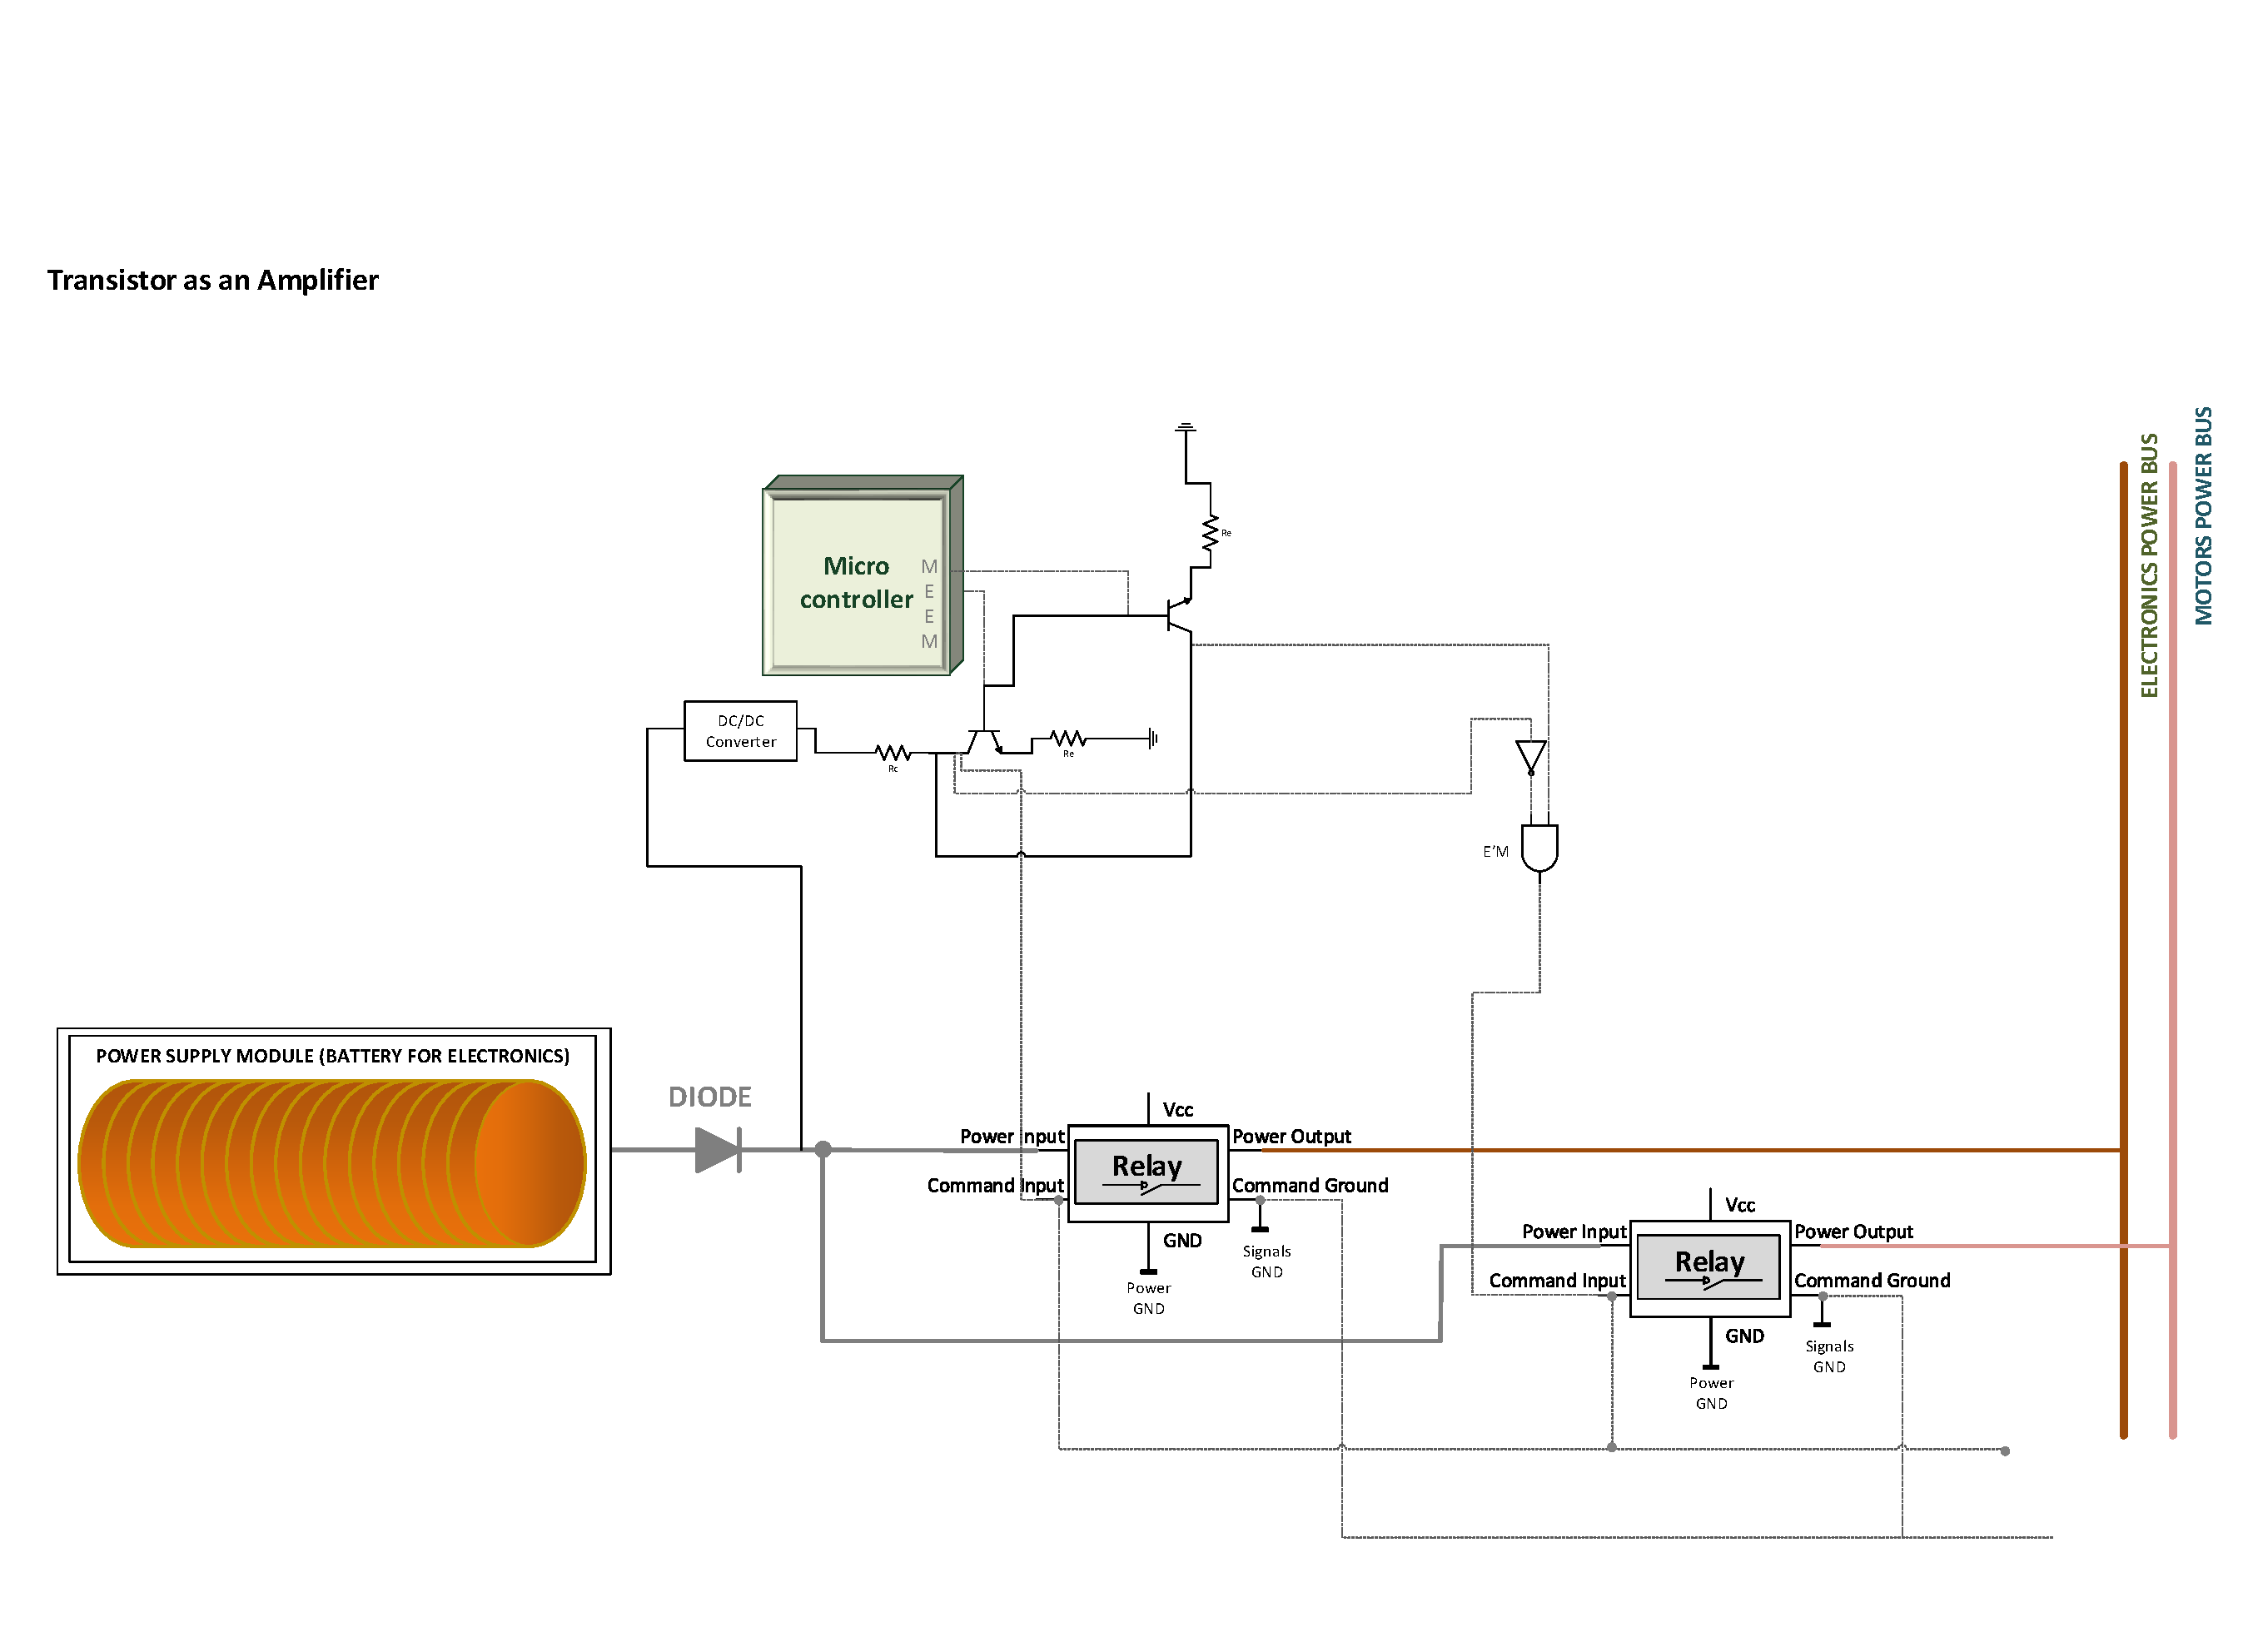
\includegraphics[width=1\columnwidth]{figs/tables/geralblockPS3.pdf}\\
  \caption[Reduction of long cycle-life battery power consumption - pulling current of the DORIS batteries using transistor]{Reduction of long cycle-life battery power consumption - pulling current of the DORIS batteries using transistor.}
  \label{FIG:SUPCIRPS3}
\end{figure}
Finally, it is important to mention the activation function of the power managing microcontroller. The robot could be deactivated by Wi-Fi through ROS system and the embedded computers would be turned off. However, the microcontroller could be accessible via Ethernet and reactivate the entire system. This procedure, using a standby microcontroller, aims economic consumption of DORIS.